\documentclass[11pt,letterpaper]{article}

\usepackage[margin=1in,letterpaper]{geometry}
\usepackage[T1]{fontenc}
\usepackage[utf8]{inputenc}
\usepackage{times}
\usepackage{amsmath}
\usepackage{amssymb}
\usepackage{array}
\usepackage{booktabs}
\usepackage{caption}
\usepackage{fancyhdr}
\usepackage{flafter}
\usepackage{float}
\usepackage{graphicx}
\usepackage{hyperref}
\usepackage{listings}
\usepackage{setspace}
\usepackage{tabularx}
\usepackage[table]{xcolor}
\renewcommand{\ttdefault}{cmtt}

\setstretch{0.95}
\raggedright
\setlength{\parindent}{0pt}
\setlength{\parskip}{0pt}
\setlength{\headheight}{14pt}
\setlength{\textfloatsep}{4pt plus 1pt minus 2pt}
\setlength{\intextsep}{4pt plus 1pt minus 2pt}
\setlength{\abovecaptionskip}{3pt}
\setlength{\belowcaptionskip}{0pt}
\setlength{\abovedisplayskip}{6pt}
\setlength{\belowdisplayskip}{6pt}
\setlength{\emergencystretch}{2em}

% Float tuning: avoid figure-only pages; keep figures near text.
\setcounter{topnumber}{2}
\setcounter{bottomnumber}{1}
\setcounter{totalnumber}{3}
\renewcommand{\topfraction}{0.92}
\renewcommand{\bottomfraction}{0.85}
\renewcommand{\textfraction}{0.06}
\renewcommand{\floatpagefraction}{0.98}

\pagestyle{fancy}
\fancyhf{}
\fancyhead[C]{CASCADE}
\fancyhead[R]{May 4, 2026}
\fancyfoot[R]{\thepage}
\renewcommand{\headrulewidth}{0pt}
\renewcommand{\footrulewidth}{0pt}

\makeatletter
\renewcommand\section{\@startsection{section}{1}{\z@}
  {0.25\baselineskip}
  {0.05\baselineskip}
  {\normalfont\large\bfseries}}
\renewcommand\subsection{\@startsection{subsection}{2}{\z@}
  {0.22\baselineskip}
  {0.05\baselineskip}
  {\normalfont\normalsize\bfseries}}
\makeatother

\definecolor{codeblue}{RGB}{0,90,160}
\definecolor{codegray}{RGB}{100,100,100}
\definecolor{codegreen}{RGB}{0,110,50}
\definecolor{codered}{RGB}{160,30,30}

\captionsetup[figure]{font=footnotesize,labelfont=bf}

\lstdefinestyle{cascade}{
  backgroundcolor=\color{gray!6},
  commentstyle=\color{codegreen},
  keywordstyle=\color{codeblue}\bfseries,
  stringstyle=\color{codered},
  basicstyle=\ttfamily\footnotesize,
  breakatwhitespace=false,
  breaklines=true,
  keepspaces=true,
  numbers=left,
  numbersep=8pt,
  numberstyle=\tiny\color{codegray},
  showspaces=false,
  showstringspaces=false,
  showtabs=false,
  tabsize=2,
  frame=single,
  rulecolor=\color{gray!40},
  captionpos=b
}
\lstset{style=cascade}
\renewcommand{\arraystretch}{1.08}
\newcommand{\cascaderepo}{https://github.com/emillambert/CASCADE}

\begin{document}
\thispagestyle{fancy}

% Single-file source of truth for the Overleaf-ready paper.
\begin{center}
{\LARGE\bfseries CASCADE: An Onboard Crop Anomaly Screening, Confirmation, and Alert Downlink Engine}\\[2pt]
{\large For Regenerative Agriculture SmallSat Missions}\\[3pt]
Emil Wes Lambert, BSc Aerospace Engineering, TU Delft \\
\smallskip
{\small Technical reviewers: Susan Steele-Dunne (TU Delft, remote sensing) \quad Stefano Speretta (TU Delft, SmallSat systems)} \\
\end{center}

\section{Introduction}

Regenerative growers, crop advisors, and food-security operators need to know which field polygons deserve scouting or targeted treatment before stress becomes visible across the whole field. Conventional workflows collect broad scenes, downlink bulk imagery, and wait for ground processing; that can be too slow or bandwidth-heavy for patch-level intervention in systems that aim to avoid blanket chemical application \cite{nasa-challenge-brief,gold-cida-seminar}. CASCADE addresses that gap as a hosted SmallSat payload that screens each pass onboard, escalates likely anomalies to confirmation, and exports a compact alert product into farm software. Evidence for the five evaluation criteria - onboard autonomy, technical feasibility, potential impact, commercial path, and reproducibility - is distributed across \S\ref{sec:solution} (SWAP + scheduler), \S\ref{sec:impact} (2014 D4 replay + Monte Carlo), \S4 (unit economics), and the MIT-licensed repository.

\section{Proposed Solution Detail}
\label{sec:solution}

CASCADE works in two onboard stages. Stage~1 runs on every pass: it measures how much greener (EVI) and wetter (NDWI) a field patch looks compared to its recent baseline, and uses those readings to update a per-patch stress probability. If that probability stays low, the pass ends there and nothing is downlinked. If it crosses a threshold, Stage~2 fires: a land surface temperature (LST) retrieval is added, and all three signals are fused into a single Crop Stress Composite (CSC) score between 0 and 1. Only patches with a CSC above the alert threshold are packaged and sent down. The algorithms follow the logic of three established NASA MODIS products (MOD13A1, MOD11A1, MOD09A1); the hosted payload flies its own multispectral and thermal sensor stack rather than the MODIS instrument itself \cite{mod13a1,mod11a1,mod09a1,mod09-guide}.

The key shift from prior onboard autonomy work is that sensing is driven by field content rather than a fixed schedule \cite{aspen-spaceops,eo1-casper-autonomous-science,eo1-autonomy,dynamic-targeting}. The satellite does more work on passes where something is changing, and less on quiet ones. The CSC equation combines vegetation loss ($\Delta$EVI), thermal rise ($\Delta$LST), and moisture loss ($\Delta$NDWI), each clipped and weighted:

\begin{equation}
\text{CSC} = 0.578 \cdot \text{clip}\!\left(\frac{\Delta\text{EVI}}{7.0\sigma_e}, 0, 1\right)
           + 0.246 \cdot \text{clip}\!\left(\frac{\Delta\text{LST}}{4.96\sigma_l}, 0, 1\right)
           + 0.176 \cdot \text{clip}\!\left(\frac{\Delta\text{NDWI}}{6.0\sigma_n}, 0, 1\right)
\label{eq:csc}
\end{equation}

where each $\Delta$ is positive when conditions are worse than the baseline and zero when they are better. The weights and saturation divisors were calibrated by a black-box search over synthetic data, minimizing false-positive rate subject to recall and resource guardrails. No real cropland data enters the calibration loop.

The scheduler picks one of four actions each pass: SKIP (battery critical), MOD13 (Stage~1 screening only, 30\,m), FUSE (full CSC computation, 10\,m confirmation), or FUSE\_PRIORITY (CSC plus priority downlink of a 4.6\,m alert tile). Each patch maintains a Beta($\alpha_i$, $\beta_i$) posterior; $\alpha_i$ increments on anomaly exceedance, $\beta_i$ otherwise, and the field-level tail statistic $\tau_{\max} = \max_i\bigl[1 - I_{0.5}(\alpha_i, \beta_i)\bigr]$, along with battery SOC and cadence $k$, drives action selection. The FUSE~$\rightarrow$~FUSE\_PRIORITY promotion additionally requires a downlink contact window and CSC above the alert threshold. A lightweight FPGA-side cloud pre-filter (Stage~0) rejects cloud-obscured frames before Stage~1 fires. This rule-based structure was chosen deliberately for flight verification traceability rather than a learned policy.


\begin{figure}[H]
\centering
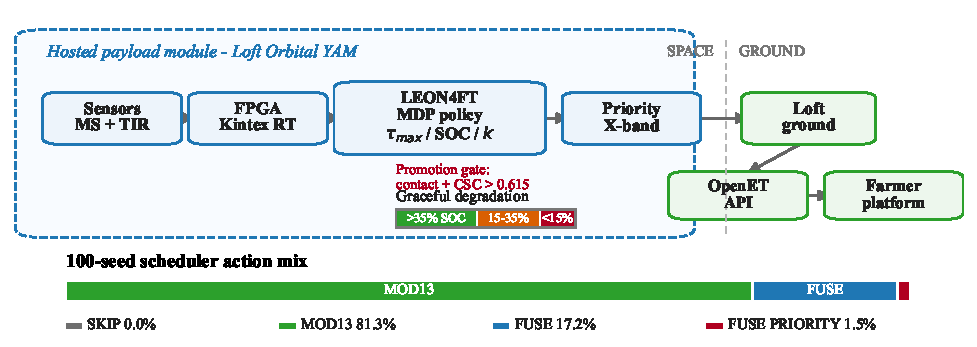
\includegraphics[width=\linewidth]{figures/architecture.pdf}
\caption{CASCADE architecture and operating mix. The policy gate uses $\tau_{\max}$, SOC, and cadence $k$; the lower bar reports the 100-seed mean actions.}
\label{fig:architecture}
\end{figure}

The spacecraft role is a hosted payload module within a Loft Orbital Yet Another Mission (YAM) bus (assumed integration baseline; no hosted-payload slot contracted at TRL~3). The FPGA performs radiometric preprocessing and per-pixel CSC computation, then transfers frames to the LEON4FT over AXI4-Stream (budgeted under 1 ms). CSC is evaluated as a pass-to-pass relative anomaly detector rather than a fully atmosphere-corrected retrieval. The selected flight part is Kintex UltraScale XQR (XQRKU060) from AMD's radiation-tolerant XQR family \cite{amd-xqr}; the SWAP budget therefore describes the payload module itself, not the host spacecraft.

Operational degradation is explicit. Between 15\% and 35\% battery state of charge, CASCADE preserves Stage~1-only screening; below 15\%, it drops to alert storage and downlink only. This satisfies the challenge requirement to degrade gracefully under onboard resource stress \cite{nasa-challenge-brief}. Processor utilization remains below the worst-case ceiling and preserves margin for RTOS and fault-handling overhead.

Each alert packet contains a geo-tagged field-patch polygon, CSC severity score, anomaly components, timestamp, pass ID, and a confidence flag from consecutive confirming passes. Escalated alert tiles are compressed onboard using CCSDS 122.0 wavelet coding with a planning assumption of roughly 2.5:1, reducing a nominal 8.4\,MB/km$^2$ native alert stream to about 3.36\,MB/km$^2$ delivered before packetization \cite{esa-cwicom}. Per-patch geolocation is derived from bus ephemeris and attitude solutions and remains inside the 30\,m screening-resolution target. Packets move through Loft Orbital's ground network to farm software as read-only geo-tagged overlays via the OpenET-linked API. Even at TRL~5, CASCADE will not write spray prescriptions back into Climate FieldView or John Deere Operations Center equipment controllers. The latency budget is decomposed into a $\leq$90 min space segment to first ground contact and a $\leq$6 h baseline / $\leq$1 h stretch target from acquisition to appearance in the grower tool.

\section{Potential Impact}
\label{sec:impact}

The unchanged production-calibrated scheduler was tested against the 2014 California D4 Exceptional Drought; the San Joaquin Valley's most severe USDA Drought Monitor event \cite{drought-monitor-2014}, with Westlands under 0\% surface-water allocation for the full water year \cite{westlands-zero-alloc}. AppEEARS V061 MOD13A1, MOD11A1, and MOD09A1 subsets over the Westlands irrigated-farmland core ($36.55^\circ$ -- $36.65^\circ$~N, $120.45^\circ$ -- $120.55^\circ$~W) were aligned to a 1~km grid, collapsed to median clear-sky LST and NDWI over 16-day windows, and replayed with the production-calibrated policy (alert threshold 0.615, unmodified) \cite{mod13a1,mod11a1,mod09a1,mod09-guide}. Across 6 valid post-warmup windows, the replay issued six FUSE\_PRIORITY alerts at every active window: peak CSC 0.869 on 13~August 2014 at 85.2\% mean valid coverage, first detection on 28~July, 41 days into the active observation window. As a quiet-season complement, the same pipeline over June through October 2024 issued seven FUSE windows, zero FUSE\_PRIORITY alerts, and peak CSC 0.412 at 99.5\% valid coverage, with no parameter adjustment.

A 100-seed Monte Carlo benchmark provides the statistical complement. Each seed runs 120 orbital passes over 500 field patches, with 21 injected anomaly events and 9 benign confounders per seed, and an average of 36.7 cloud-obscured passes. The belief gate means the satellite is doing full fusion (FUSE or FUSE\_PRIORITY) on only about 19\% of passes; the other 81\% end at Stage~1 screening.

The headline results across 100 seeds: 99.05\% downlink reduction versus raw (95\% CI 99.04--99.07\%), 38.3\% energy saving (95\% CI 38.20--38.38\%), 100.0\% anomaly recall, and 0.6\% false-positive rate. Recall is held as a hard constraint; the calibration minimizes false positives subject to catching every event so the 100\% interval is expected. The interesting tradeoff is the threshold: at 0.40 the FP rate climbs to 1.52\% while recall stays perfect; at 0.65 recall slips to 99.3\%; at 0.70 it falls to 84.6\%. The calibrated value 0.615 sits at the knee of that curve. Removing the Bayesian belief gate entirely (no-belief ablation) matches the FP rate but burns 76.2\% seasonal compute and 587.9\,MB of downlink versus 49.2\% and 136.3\,MB for full CASCADE; the belief gate is what makes the efficiency gains possible.

\begin{table}[H]
\centering
\caption{Baseline comparisons under the synthetic Monte Carlo benchmark.}
\label{tab:baselines}
\small
\setlength{\tabcolsep}{4pt}
\renewcommand{\arraystretch}{1.1}
\begin{tabularx}{\linewidth}{@{}>{\raggedright\arraybackslash}p{3.15cm}*{5}{>{\centering\arraybackslash}X}@{}}
\toprule
Variant & Downlink red.\,$\downarrow$ & MB\,$\downarrow$ & Recall\,$\uparrow$ & FP\,$\downarrow$ & Compute\,$\downarrow$ \\
\midrule
Raw downlink & 0.0\% & 14400.0 & 100.0\% & 0.5\%\textsuperscript{a} & N/A \\
Fixed-period onboard & 95.8\% & 610.9 & 100.0\% & 0.5\% & 92.5\% \\
EVI-only threshold & 96.2\% & 542.4 & 100.0\% & 2.3\% & 39.2\% \\
No-belief CASCADE & 95.9\% & 587.9 & 100.0\% & 0.5\% & 76.2\% \\
\rowcolor{green!8} Full CASCADE & 99.05\% & 136.3 & 100.0\% & 0.6\% & 49.2\% \\
\bottomrule
\end{tabularx}
\par\vspace{2pt}
\parbox{\linewidth}{\footnotesize \textsuperscript{a}Raw downlink FP is the same offline benchmark classifier applied post hoc to the full stream, not an onboard decision.}
\end{table}

\begin{figure}[H]
\centering

\includegraphics[width=\linewidth]{figures/additional_ablation_curves.pdf}
\caption{Additional ablations. Panel~(a): threshold sweep showing operating point at 0.615 and the NDWI-removed FP penalty, with CSC saturation sensitivity overlaid as a callout. Panel~(b): sparse screening cadence holds recall above 99.6\% while compute falls monotonically with stride.}
\label{fig:additional-ablations}
\end{figure}

\begin{figure}[H]
\centering
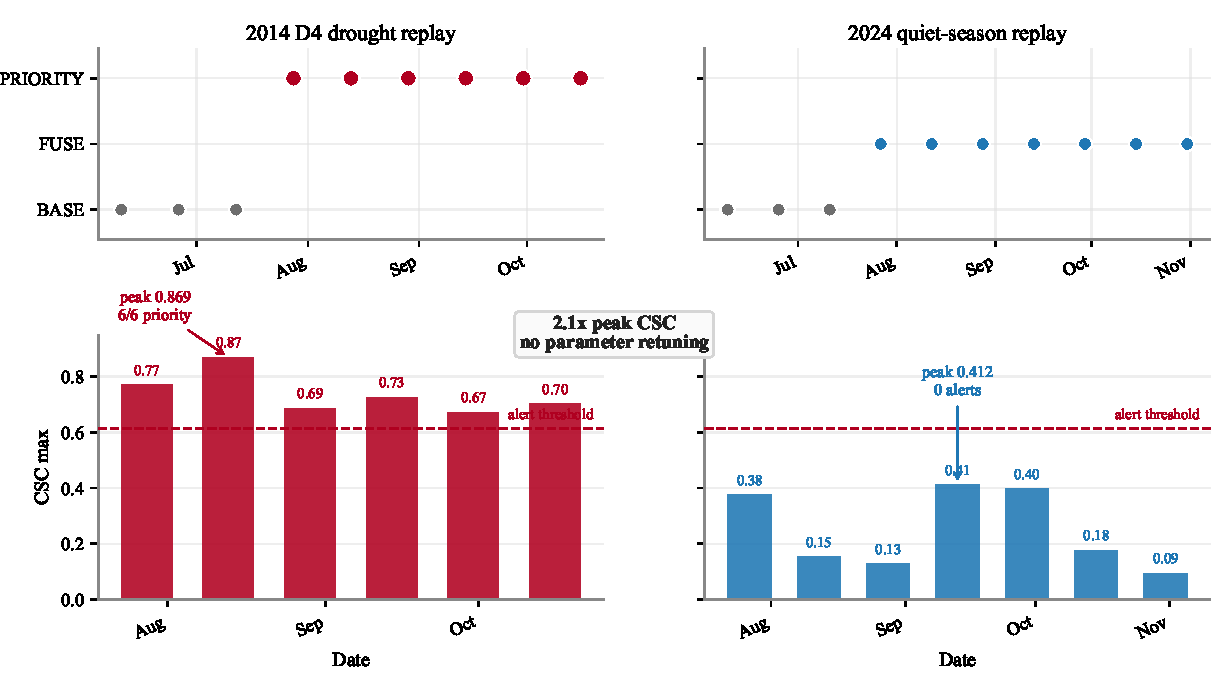
\includegraphics[width=0.98\linewidth]{figures/action_timeline_westlands_split.pdf}
\caption{Westlands replay: 2014 D4 Exceptional Drought (left) versus 2024 quiet season (right), identical parameters. Every post-warmup window triggers FUSE\_PRIORITY in 2014 (peak CSC 0.869); the 2024 season stays below the alert threshold (peak CSC 0.412) — a 2.1$\times$ separation with no retuning.}
\label{fig:action-timeline}
\end{figure}

CASCADE flags stress anomalies regardless of cause; etiology disambiguation (drought vs.\ pathogen vs.\ nutrient) is the role of downstream confirmation by scouts or hyperspectral assets \cite{gold-cida-seminar}. For a 500 ha regenerative tomato operation, confining treatment to the $\sim$8\% of field area flagged per event yields a modeled chemical-spend reduction of roughly \$34{,}000--\$55{,}000/season versus blanket application (based on UC Cooperative Extension disease-control line items of \$74--119/ha/season \cite{uc-tomato-cost}). The same triage logic applies across anomaly types: the onboard architecture changes how scarce intervention effort is directed.

\section{Team Experience and Market Evaluation}

Emil Wes Lambert is completing a BSc in Aerospace Engineering at TU Delft, with coursework in spacecraft systems, Attitude and Orbit Control Systems (AOCS), mission analysis, and embedded flight software. At AeroDelft, a student team building a liquid-hydrogen-electric aircraft, he has led finance, legal, and partnerships work across AeroDelft's 50+ industry partners (including KLM, Airbus, and the Ministry of Defence), and secured AeroDelft’s participation in a €73M hydrogen aviation consortium under the National Growth Fund. That background supports CASCADE's SWAP realism, AIST-track funding strategy, and commercial positioning; the first commercial system sells an onboard scheduler plus alert overlay, not closed-loop agronomic prescriptions. Technical review was provided by Susan Steele-Dunne (TU Delft, remote sensing and vegetation index retrieval) and Stefano Speretta (TU Delft, SmallSat systems and embedded flight software).

The commercialization path is illustrative rather than predictive. Westlands anchors NASA-data validation; the first commercial wedge is European irrigated and high-value-crop agriculture, where parcel-level public data (BRP/IACS, gridded weather, soil cadastre) and policy demand (CAP area monitoring, regenerative-agriculture schemes) make the time-to-paid-pilot shortest. From a Benelux beachhead CASCADE scales into the wider EU, the U.S. irrigated base, and global commercial markets with region-specific CSC recalibration \cite{usda-2022,eurostat-farms,fao-aquastat}. A parallel non-commercial track delivers zero-cost alert data to subsistence-scale growers through World Bank, FAO, and CGIAR-supported programmes; this track carries no commercial TAM but generates continental-scale coverage, independent validation datasets, and food-security impact credentials that reinforce the commercial path and reduce pesticide use where cost recovery is impossible. The commercial economics use a low/design-to-cost case with a \$4/ha/year alerting-overlay reference price as an illustrative floor; the realistic revenue mix layers API-and-embed distribution through advisors and crop-software platforms with enterprise contracts to processors (supply-risk), insurers (parametric data feed), and MRV programmes, plus a Year~2 soil-carbon MRV add-on aligned to Verra VM0042-style workflows \cite{verra-vm0042}. At the Y5 coverage in Table~\ref{tab:unit-econ}, about 18\,Mha, the same benchmark-style treatment-confinement assumption implies roughly \$1--2\,B/season in avoidable spend; this is an impact lens, not a revenue forecast.

\begin{table}[H]
\centering
\caption{Illustrative CASCADE rollout. Y1 anchor pilot (EU or SJV) is validation-geography-dependent; subsequent scale follows irrigated-area data \cite{usda-2022,eurostat-farms,ana-atlas,fao-aquastat}.}
\label{tab:unit-econ}
\footnotesize
\setlength{\tabcolsep}{3pt}
\renewcommand{\arraystretch}{1.0}
\begin{tabular*}{\linewidth}{@{\extracolsep{\fill}}l>{\raggedright\arraybackslash}p{2.75cm}>{\raggedright\arraybackslash}p{2.35cm}>{\raggedright\arraybackslash}p{2.35cm}c>{\raggedleft\arraybackslash}p{1.35cm}>{\raggedleft\arraybackslash}p{1.65cm}@{}}
\toprule
Year & Milestone & Geography & Coverage & Scale & Revenue & Op. margin \\
\midrule
Y1 & Anchor pilot & EU or SJV & $\leq$5\% region & \makebox[1.35cm][l]{\textcolor{codeblue}{\rule{0.18cm}{0.7ex}}} & \$0.20\,M & grant-funded \\
Y2 & Benelux + CA scale & EU + California & EU wedge + SJV & \makebox[1.35cm][l]{\textcolor{codeblue}{\rule{0.58cm}{0.7ex}}} & \$1.70\,M & 17.1\% \\
Y3 & EU + U.S. national & EU + U.S. irrigated & 11.0\% US & \makebox[1.35cm][l]{\textcolor{codeblue}{\rule{0.94cm}{0.7ex}}} & \$10.62\,M & 60.4\% \\
Y4 & EU expansion + intl.\ org pilots\textsuperscript{b} & EU + U.S. & 35.1\% EU & \makebox[1.35cm][l]{\textcolor{codeblue}{\rule{1.12cm}{0.7ex}}} & \$27.62\,M & 68.1\% \\
Y5 & Global commercial & Global (commercial) & 6.0\% global & \makebox[1.35cm][l]{\textcolor{codeblue}{\rule{1.32cm}{0.7ex}}} & \$76.50\,M & 70.7\% \\
\bottomrule
\end{tabular*}
\par\vspace{1pt}
\parbox{\linewidth}{\footnotesize Scale bar is log-scaled covered hectares (50\,kha to 18\,Mha). \textsuperscript{b}Intl.\ org pilots (World Bank, FAO, CGIAR) are grant/donor funded with zero commercial TAM; coverage and validation data feed back into the commercial path.}
\end{table}

These are API integration targets, not committed channels. Y1 is modeled as a co-funded bridge-to-MVP year, executable on a NASA AIST/SBIR track \cite{nasa-aist,nasa-sbir} or an ESA InCubed / Horizon Europe-equivalent track, with the choice driven by which side of the Atlantic the first anchor pilot lands; break-even occurs at Y2 and 400\,kha in the low case, and Y3 and 2.5\,Mha in the base/high cases.

The near-term product is the grower-facing polygon overlay; insurance scoring and food-security rasters are later extensions. Agriculture is the entry market, but the same Beta-posterior and threshold structure operates over any anomaly index without changing the action set or the SWAP budget: swapping CSC for a fuel-moisture, flood-inundation, or urban heat-island index extends CASCADE to wildfire, flood-front, or city-scale monitoring; wildfire alone points toward a market measured in the tens of billions of dollars \cite{fire-detection-market}.

\section{Expected Next Steps}
\label{sec:next}

CASCADE is currently TRL 3: the scheduler, CSC calibration, SWAP closure, and real-scene replay are software-demonstrated but not yet on flight-like compute. Next is TRL~4 hardware-in-the-loop on a LEON4FT-class processor under NASA AIST, using the replayed EarthData scene set and Kintex UltraScale XQR bitstream verification for the FPGA-side Stage~0 cloud pre-filter (\S\ref{sec:solution}). The TRL 5 path is a Loft Orbital hosted-payload pilot with external Y1/agronomy validation; finalist prep is a live non-Westlands MODIS replay plus a first-pass Loft cost estimate.


\section{Conclusion}

\label{chapter:conclusion}

CASCADE operationalizes onboard crop-anomaly triage on constrained SmallSats. The core engineering result is a belief-gated two-stage scheduler that reduces downlink volume by 99.05\% and energy consumption by 38.3\% relative to raw collection, while holding 100\% anomaly-event recall across a 100-seed Monte Carlo benchmark. Validated against archival MODIS data, the unchanged production-calibrated policy issued six FUSE\_PRIORITY alerts across every post-warmup window of the 2014 California D4 Exceptional Drought and zero alerts in the 2024 quiet season, a 2.1$\times$ peak-CSC separation with no parameter adjustment.

The broader contribution is precision triage: read-only geo-tagged alert overlays confine treatment to the $\sim$8\% of field area under confirmed stress, connecting SmallSat Earth observation directly to regenerative agriculture's goal of reducing blanket chemical application. The scheduler is MIT-licensed and anomaly-index agnostic; TRL-4 hardware-in-the-loop under NASA AIST is the next step toward a Loft Orbital hosted-payload demonstration.

\newpage
\begingroup
\footnotesize
\bibliographystyle{unsrt}
\bibliography{references}
\endgroup

\end{document}
